It is often claimed that Einstein ``abolished the æther'' in his theory of relativity. While this has become a popular shorthand in both educational and philosophical discussions, it severely oversimplifies Einstein's actual position~\cite{einstein1920aether}. In his early work (1905), Einstein dispensed with the notion of the luminiferous æther as a mechanical carrier of electromagnetic waves. Yet, in later writings—most notably his 1920 lecture at Leiden—he reintroduced a more subtle concept of æther, reinterpreted within the context of spacetime geometry.
For historical quotations and their mappings to VAM dynamics, see Appendix~\ref{appendix:einstein}.


This paper revisits Einstein’s evolving perspective on the æther and evaluates its compatibility with the comprehensive Vortex Æther Model (VAM) program, as presented in the recent VAM master paper~\cite{VAM-8} and its companion studies.


VAM proposes that the æther is a structured, incompressible fluid medium whose knotted vorticity fields underlie all known phenomena—gravitation, inertia, time, quantum behavior, and cosmological structure.

\textit{This framework has been previously applied to the photon as a topological vortex tube in a structured æther, offering a physical model for electromagnetic propagation and quantized energy flow~\cite{VAM-17.1}.}

The present work extends this ontological structure to spacetime geometry and time itself, positioning VAM as a coherent alternative to standard field-theoretic approaches.

Through a topological and dynamical synthesis, VAM provides not only a conceptual bridge but also explicit, testable predictions that unite historical field theory with contemporary advances in fundamental physics.~\cite{VAM-11, VAM-15}, and connects with modern analogue gravity approaches where fluid systems mimic general relativistic metrics~\cite{barcelo2005}.This intellectual trajectory is summarized in Figure~\ref{fig:history-temporal-ontology}, which maps key milestones in the conceptualization of time—from pre-Socratic polarity and Augustine’s introspective present to Einstein’s relativized geometry and the layered temporality proposed in VAM.

\begin{figure}[htbp]
      \centering
    \scriptsize
    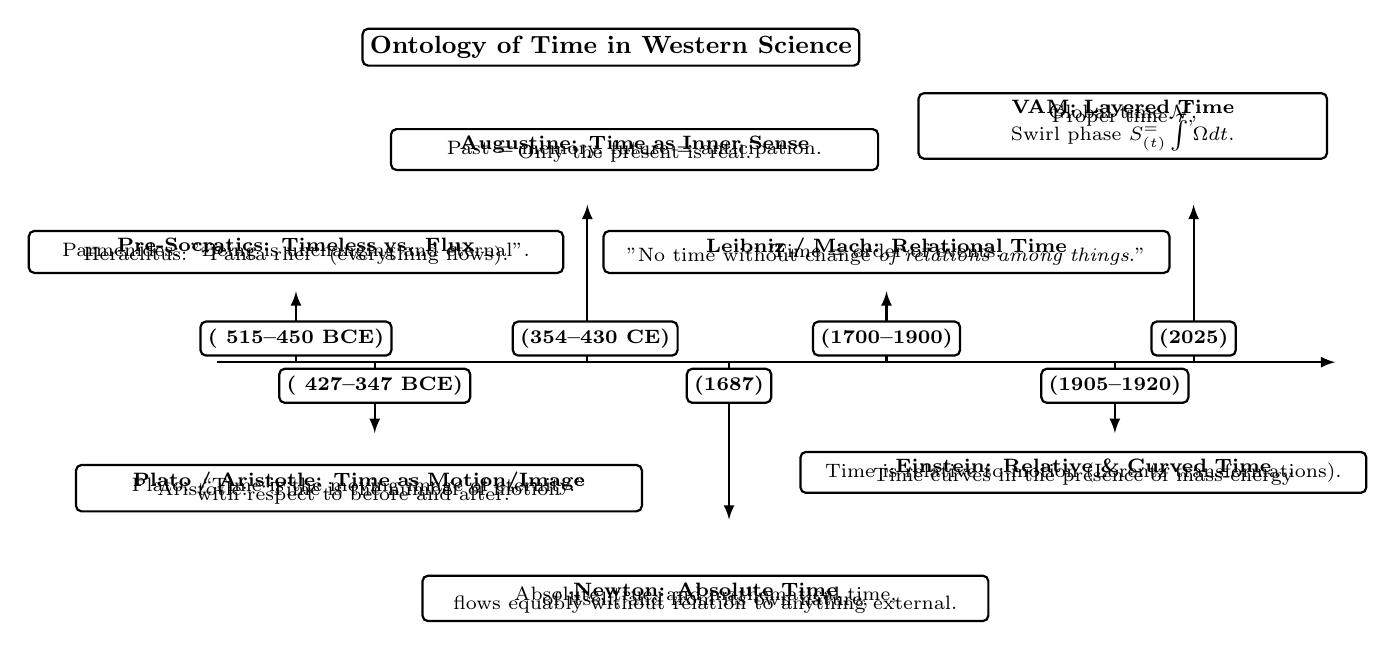
\begin{tikzpicture}[node distance=3.5cm, every node/.style={font=\scriptsize}, >=latex]
    \scriptsize

    % Timeline base
    \draw[->, thick] (-1,0) -- (13.2,0);

    % Arrows above timeline (short, as requested)
    \draw[->, thick] (0,0) -- (0,0.9);       % Pre-Socratics
    \draw[->, thick] (3.7,0) -- (3.7,2.0);   % Augustine
    \draw[->, thick] (7.5,0) -- (7.5,0.9);   % Einstein
    \draw[->, thick] (11.4,0) -- (11.4,2.0); % VAM

    % Arrows below timeline (short, as requested)
    \draw[->, thick] (1.0,0) -- (1.0,-0.9);     % Plato/Aristotle
    \draw[->, thick] (5.5,0) -- (5.5,-2.0);     % Newton
    \draw[->, thick] (10.4,0) -- (10.4,-0.9);     % Leibniz/Mach

        %--- Root title cards (above timeline) ---
    \node[draw, thick, rounded corners=2pt, fill=white, align=center, font=\bfseries ] at (0, .3)   {(~515–450 BCE)};
    \node[draw, thick, rounded corners=2pt, fill=white, align=center, font=\bfseries ] at (3.8, .3) {(354–430 CE)};
    \node[draw, thick, rounded corners=2pt, fill=white, align=center, font=\bfseries ] at (7.5, .3) {(1700--1900)};
    \node[draw, thick, rounded corners=2pt, fill=white, align=center, font=\bfseries ] at (11.4, .3){(2025)};

    %--- Root title cards (below timeline) ---
    \node[draw, thick, rounded corners=2pt, fill=white, align=center, font=\bfseries ] at (1.0,- .3) {(~427–347 BCE)};
    \node[draw, thick, rounded corners=2pt, fill=white, align=center, font=\bfseries ] at (5.5,- .3) {(1687)};
    \node[draw, thick, rounded corners=2pt, fill=white, align=center, font=\bfseries ] at (10.4,- .3) {(1905--1920)};

    % Label
    \node[draw, thick, fill=white, rounded corners=2pt, font=\small] at (4,4.0) {\textbf{Ontology of Time in Western Science}};

    % Ancient Greek: Parmenides / Heraclitus
    \node[draw, rounded corners=2pt, thick, align=center, fill=white, text width=6.6cm] at (0,1.4) {
    \textbf{Pre-Socratics: Timeless vs. Flux}  \\[-0.8em]
    Parmenides: "Being is unchanging and eternal".  \\[-0.8em]
    Heraclitus: “Panta rhei” (everything flows).
    };

    % Plato / Aristotle
    \node[draw, rounded corners=2pt, thick, align=center, fill=white, text width=7cm] at (0.8,-1.6) {
    \textbf{Plato / Aristotle: Time as Motion/Image}  \\[-0.8em]
    Plato: “Time is the moving image of eternity.” \\[-0.8em]
    Aristotle: “Time is the number of motion \\[-0.8em]
    with respect to before and after.”
    };

    % Augustine
    \node[draw, rounded corners=2pt, thick, align=center, fill=white, text width=6cm] at (4.3,2.7) {
    \textbf{Augustine: Time as Inner Sense}  \\[-0.8em]
    Past = memory, future = anticipation. \\[-0.8em]
    Only the present is real.
    };

    % Newton
    \node[draw, rounded corners=2pt, thick, align=center, fill=white, text width=7cm] at (5.2,-3.0) {
    \textbf{Newton: Absolute Time}  \\[-0.8em]
    Absolute, true, and mathematical time, \\[-0.8em]
    of itself, and from its own nature, \\[-0.8em]
    flows equably without relation to anything external.
    };


    % Relationalists: Leibniz / Mach
    \node[draw, rounded corners=2pt, thick, align=center, fill=white, text width=7cm] at (7.5,1.4) {
    \textbf{Leibniz / Mach: Relational Time}  \\[-0.8em]
    Time = order of events.  \\[-0.8em]
    "No time without change \textit{of relations among things}."
    };

    % Einstein
    \node[draw, rounded corners=2pt, thick, align=center, fill=white, text width=7cm] at (10.0,-1.4) {
    \textbf{Einstein: Relative \& Curved Time}  \\[-0.8em]
    Time is relative to motion (Lorentz transformations). \\[-0.8em]
    Time curves in the presence of mass-energy
    };


    % VAM
    \node[draw, rounded corners=2pt, thick, align=center, fill=white, text width=5cm] at (10.5,3.0) {
    \textbf{VAM: Layered Time}  \\[-0.8em]
    Global time \( \mathcal{N} \), \\[-0.8em]
    Proper time \( \tau \),  \\[-0.4em]
    Swirl phase \( S_\text{(t)}^\circlearrowleft = \int \Omega dt \).
    };
    \end{tikzpicture}
      \caption{\textbf{Historical progression of time concepts from metaphysics to field theory.} The diagram traces Western ontologies of time—from eternal being and motion-based time, through Newtonian absolutes and Einsteinian relativity, to VAM’s layered temporal framework: global æther time \( \mathcal{N} \), proper time \( \tau \), and internal swirl phase \( S_\text{(t)}^\circlearrowleft \). This continuum repositions time as a structured, fluid-dynamical hierarchy.}

      \label{fig:history-temporal-ontology}
\end{figure}

Unlike modern field theories that eliminate any underlying substrate, VAM embraces the æther as the unified, dynamically active fabric through which geometry, force, and phase propagate—resonating with dynamical 3-space approaches that reinterpret space itself as a flowing medium~\cite{cahill2003dynamical}.

This work also answers a broader philosophical concern raised in recent critiques of modern theoretical physics. Hossenfelder argues that a disproportionate emphasis on mathematical elegance has led to speculative models lacking physical transparency and empirical anchoring~\cite{hossenfelder2018lost}. The Vortex Æther Model (VAM), by contrast, re-centers physics on a physically meaningful substrate—modeled explicitly as a quantized fluid medium—and derives its equations from conservation laws, vortex dynamics, and experimentally accessible analog systems. In doing so, VAM aims to reconnect theoretical inquiry with empirical testability and conceptual coherence.

The goal of this study is twofold: first, to clarify Einstein’s nuanced philosophical stance regarding the æther—tracing its transformation from a mechanical substrate to a geometric and energetic foundation for field theory; and second, to construct a rigorous conceptual and mathematical bridge between this historical lineage and contemporary physics. This aligns with modern investigations into spacetime microstructure and emergent geometry from more fundamental constituents~\cite{hossenfelder2018lost}.


This bridge is now rendered concrete through the comprehensive VAM series (see ~\cite{VAM-8} for full derivations), which provides:

\begin{itemize}
    \item Explicit mathematical derivations of the foundational equations of VAM, including the emergence of gravitational, inertial, and quantum effects from topological swirl dynamics and the formal structure of multimodal time;
    \item A master equation for particle masses and a complete knot-based taxonomy, unifying leptons, baryons, and their quantum numbers (see Sec.~\ref{fig:taxonomy}, ~\cite{VAM-8}, ~\cite{VAM-11}) This continues the legacy of vortex-knot models in fluid mechanics and their application to particle structure~\cite{knot_theroy_in_fluid};
    \item Empirical benchmarking against classical and modern tests, as well as predictions for new phenomena in quantum gravity, cosmology, and particle physics (see ~\cite{VAM-8}, ~\cite{VAM-12}, ~\cite{VAM-15});
    \item A unified topological fluid-dynamical Lagrangian connecting all known interactions to a single underlying vortex æther (see ~\cite{VAM-14}).
\end{itemize}

These ideas resonate with entropic and emergent gravity theories that derive gravitation from statistical or information-theoretic considerations~\cite{Verlinde2011}.

Together, these advances transform the æther hypothesis from historical curiosity into a predictive, mathematically mature, and experimentally relevant framework for fundamental physics. A similar perspective is adopted in condensed matter analogs of quantum vacuum, notably in superfluid helium models of emergent spacetime~\cite{volovik2003universe}.


VAM now extends beyond gravity to encompass a unified, topological account of particle masses, quantum phenomena, and cosmology.

A historical overview of ætheral and vortex field theory—from Helmholtz to VAM—is provided in Appendices~\ref{appendix:helmholtz}–\ref{appendix:einstein}, alongside a mapping of Einstein’s quotations to the specific dynamical structures in VAM. This lineage incorporates classical results from vortex ring dynamics and stability~\cite{morris1977vortex}, now reinterpreted through the lens of topological swirl formalism.


\begin{figure}[htbp]
    \centering
    \vspace{1em}
    \noindent\textbf{Lineage of Æther and Vortex Physics:}

    \[
        \fbox{\makebox[2.2cm][c]{Helmholtz}} \;\longrightarrow\;
        \fbox{\makebox[2.2cm][c]{Kelvin}} \;\longrightarrow\;
        \fbox{\makebox[2.2cm][c]{Maxwell}} \;\longrightarrow\;
        \fbox{\makebox[2.2cm][c]{Einstein}} \;\longrightarrow\;
        \fbox{\makebox[2.2cm][c]{VAM}}
    \]

    \vspace{0.2em}
    {\scriptsize
    \textit{
        Conservation of vorticity $\;\rightarrow\;$ Topological atoms $\;\rightarrow\;$ Field stress in æther $\;\rightarrow\;$ Geometric æther $\;\rightarrow\;$ Unified Vortex-fields}
    }

    \vspace{0.2em}
    \[
        \fbox{\makebox[2.2cm][c]{(1858)}} \;\longrightarrow\;
        \fbox{\makebox[2.2cm][c]{(1867--1890)}} \;\longrightarrow\;
        \fbox{\makebox[2.2cm][c]{(1875--1878)}} \;\longrightarrow\;
        \fbox{\makebox[2.2cm][c]{(1920--1924)}} \;\longrightarrow\;
        \fbox{\makebox[2.2cm][c]{(2012--2025)}}
    \]

    \caption{\textbf{Intellectual lineage of vortex and æther physics,} from Helmholtz’s vorticity conservation to the Vortex Æther Model (VAM).}
    \label{fig:lineage-aether-vortex}
\end{figure}